
% bc.tex

\documentclass[10pt,a4paper]{article}
%\usepackage[czech]{babel}
\usepackage[utf8]{inputenc}
\usepackage[margin=100pt]{geometry}
    
\usepackage{graphicx}   % Import pictures
\usepackage{multicol}
\usepackage{caption}
\usepackage{subcaption}
%\usepackage{csquotes}

\usepackage[backend=biber, sorting=none]{biblatex}
\addbibresource{bc.bib}
    
\begin{document}
  %\pagenumbering{gobble}

  \begin{titlepage}

  \begin{center}
  % Headings
  \textsf{\LARGE \bfseries Brno University of Technology}\\[0.5cm]
  \textsf{\large \bfseries Faculty of Information Technology}\\[9cm]
  
  % Title - lines
  \textsf{ \Large \bfseries Classification of a Situation Using Signals from PIR-Sensors}\\[0.3cm]
  \textsf{ \bfseries Martin Beneš}\\[1cm]
  \end{center}
  \end{titlepage}
  \newpage

  % table of contents
  \tableofcontents
  \newpage

  \section{Physics Basis}
  Every object whose temperature is higher than absolute zero ($T_{obj}>0~K\equiv -273.15^{\circ}C$)
  emits radiation. It is caused by a charged subatomical particles (electrons, protons) that are
  undergoing an acceleration, emitting an energy in a form of photon - electromagnetic radiation.
  
  Electromagnetic waves are being divided into categories according to their usage by the frequency $f$
  or wavelength $\lambda$. These characteristics are due to a constant travel speed proportional,
  $f=\frac{c}{\lambda}$, where $c=3\cdot10^{8}~m\cdot s^{-1}$ is a speed of light. With increasing
  wavelength~$\lambda$ it is gamma, X-rays, ultraviolet (UV), visible light, infrared (IR) and
  radio waves, this division is shown in the image \ref{fig:spectrum}.

  \begin{figure}[h!]
    \begin{center}
      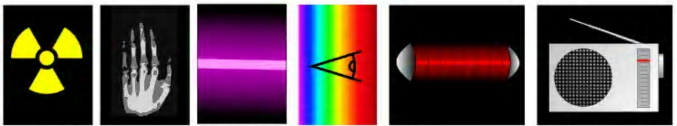
\includegraphics[width=0.5\textwidth]{spectrum.png}
      \caption[title=Obrazek]{Electromagnetic spectrum\label{fig:spectrum} \cite{IZGcolors}}
    \end{center}    
  \end{figure}

  \section{Zdroj}
  Therefore, infrared rays are surrounding us during our whole life, human skin is very sensitive to it,
  we sense it as a warmth. Energy of such radiation is computed as $$W_e=h\cdot f$$ where $W_e$ corresponds
  to a photon energy, $f$ is the frequency of the electromagntic radiation and $h=6.63\cdot10^{-34}~J\cdot s $
  is Planck constant.



  Human body with temperature around $36.5^\circ C$ radiates mainly at wavelength around $10~\mu m$,
  our skin is to that kind of radiation sensitive, we can feel it as a warmth.


  
  PIR ({\it passive infrared}) sensor is an electronic device that scans electromagnetic
  radiation at~wavelength $\lambda\in<700~nm;2.5~mm>$ aka frequency $f\in<120~MHz;430~THz>$.

  

  Infračervené záření se tedy vyskytuje běžně kolem nás a naše tělo jej vnímá jako teplotu. Energie
  takového záření (tzv. zářivá energie) se spočítá jako $W_e=h\cdot f$, kde $f$ je kmitočet záření
  a $h=6.63\cdot10^{-34}~J\cdot s $ je Planckova konstanta. \cite{WikipediaInfrared}

  \section{Infračervené detektory}
  \subsection{Inspirace přírodou}
  Některé organismy jsou schopny vnímat infračervené záření a tím zvyšovat svoji šanci na přežití.
  Jedním z nich jsou někteří hadi (krajty, chřestýši, hroznýši...), kteří mají v obličeji velmi citlivé
  termoreceptory, které jim pomáhají v lovu teplokrevných živočichů. Díky jejich směrové citlivosti
  a toho, že jejich více, mohou přesně odhadovat směr a vzdálenost, kde se nachází kořist. \cite{SnakeInfrared}
  Živočichové, kteří se živí krví, např. upír obecný nebo jihoamerická ploštice Triatoma infestans,
  používají termoreceptory, aby poznali místo, kde je céva a kam tedy kousnout.

  \subsection{Konstrukce}
  Při snímání je možné využít hned několik látek, které reagují na teplotu, a to tak, že je možné
  toto chování co nejpřesněji snímat elektrickým obvodem a vyhodnocovat počítačem. Podle
  charakteru jejich chování se detektory, které toho využívají, dělí na jednotlivé typy.
  {\it Bolometry} využívají změnu elektrického odporu vlivem ohřevu odporového elementu
  absorbovaným vstupním zářením. {\it Termoelektrické detektory} snímají změnu termoelektrického
  napětí dvojice vodičů vlivem rozdílu teplot mezi meřícím (ozářeným) a srovnávacím (zatemněným)
  spojem. {\it Pyroelektrické detektory} jsou založeny na elektrostatické polarizaci, měnící se při
  změně teplot. \cite{DetectorsBook}

  Stejně tak, jako chřestýši jsou schopni určovat přesnou pozici kořisti, je pro reálné využití detektoru
  při snímání a rozpoznávání třeba dosáhnout směrové citlivosti. Proto se používá podobná technika jako
  u fotoaparátů, jednotlivé jednoduché snímače se umístí do matice a data, které tyto snímače produkují,
  jsou poté řetězcem výpočetních jednotek zpracovávány do požadovaného výstupního formátu.
  
  \section{Klasifikace}
  Klasifikace je druh problému, kteří řeší, do které z tříd (kategorií) dat patří nové pozorování.
  Aby bylo možné klasifikaci provádět na počítači, je nutné reprezentovat pozorování kvantitavně,
  a to buď strukturálně, nebo - a to je ten častější způsob - za pomocí příznaků ({\it features}).

  \subsection{Klasifikátor}
  Základem klasifikátoru je strojové učení. Na počátku se vystaví systém, který se naučí rozpoznávat
  dané objekty, které po něm chceme, pomocí množiny trénovacích dat. Snaží se o maximální obecnost
  a generalizaci, přičemž současně o maximální přesnost a úspěšnost při rozpoznávání.

  \begin{figure}[h!]
    \begin{center}
      %\includegraphics[width=1\textwidth]{classification.png}
      \caption[title=Obrazek]{Klasifikační {\it pipeline}.\label{fig:classification}}
    \end{center}    
  \end{figure}

  Na obrázku \ref{fig:classification} je možné vidět, jaké kroky má proces klasifikace, a tedy
  jakými problémy je nutné se zabývat při vytváření klasifikačního systému.
  
  \paragraph{Segmentace}
  Přímo po nasnímání je nutné signál rozdělit na části, které se klasifikují zvlášť, jak pro
  zajištění rychlého zpracování a dostatku paměti a zdrojů, tak i pro možnost zpracovávat
  daný signál přímo {\it real-time}.

  \paragraph{Extrakce příznaků}
  Dalším krokem v posloupnosti je extrakce příznaků. Příznaky nahrazují signál na vstupu,
  a jsou jeho kvantitativním vyjádřením. Návrh pro jejich extrakci a následný proces je klíčový
  pro následující klasifikátor. Pro dobré výsledky je nutné, aby byly příznaky co možná nejvíce
  diskriminativní, tedy umožňovat rozlišení mezi třídami, invariantní vůči případným transformací
  (translaci, rotaci, změně měřítka atd.) a dekorelované, být vzájemně nezávislé. Účelem příznaků
  je snížit komplexnost a paměťovou a výpočetní složitost.

  \paragraph{Klasifikace}
  Po získání takovýchto příznaků je zpracovává klasifikační systém, který přiřazuje n-tici příznaků
  jako celek k nějaké třídě. Druhů klasifikátorů je spousta, obecně by se daly rozdělit na dvě
  skupiny - generativní a diskriminativní.
  
  Generativní klasifikátor si z trénovacích dat odvodí jejich souvislost a nalezne si reprezentaci
  třídy jako celku. Často uvažuje gaussovo rozložení dat a hledá střední hodnotu $\mu$ a varianci (rozptyl)
  $\sigma^2$ v jednom rozměru, resp. střední hodnotu $\bar{\mu}$ a kovarianční matici $\Sigma$ ve
  vícedimenzionálním prostoru.
  
  Diskriminativní klasifikátor hledí na každý vzorek zvlášť a nijak negeneralizuje. Jsou vhodnější
  pro učení s učitelem ({\it supervised learning}), generativní klasifikátory jsou více flexibilní
  a jsou lepší volbou při učení bez učitele ({\it unsupervised learning}). Výběr správného
  modelu je závislý na aplikaci.

  %Mezi nejpoužívanější generativní klasifikátory patří MAP ({\it maximum a-posteriori}), který vybíra
  %z množiny všech tříd tu, která má pro daný vektor příznaků $\bar{x}$ největší posteriorní pravděpodobnost
  %$P(C_c | \bar{x})$, tedy $$\bar{x} \rightarrow C_c \Leftrightarrow \forall C_k \in \{ C_1, C_2, ...\}:
  %P(C_c | \bar{x}) \geq P(C_k | \bar{x})$$ Dalším známým mechanismem je model GMM (Gaussian mixture
  %model), počítající s daty jako se směsí gaussovských rozložení. Apriorní pravděpodobnost $P(\bar{x})$
  %je možné zapsat $$P(\bar{x}) = \sum_{C} p(\bar{x} | C) P(C) = \sum_{C} \mathcal{N}(\bar{x}; \bar{\mu}_C,
  %\Sigma_C) P_C$$ Takovýto model je možné trénovat, např. iterativním algoritmem {\it vitebri training},
  %nebo pokročilejším algoritmem EM ({\it expectation minimalization}), který namísto tvrdých přiřazení
  %jako u vitebri training využívá vah - posteriorních pravděpodobností.

  Jeho základem je nejčastěji nějaký lineární klasifikátor (nicméně lineární v n-rozměrném prostoru),
  popř. neuronová síť\footnote{Neuronová síť je ve své podstatě vlastně jen kompozice vzájemně
  popropojovaných lineárních klasifikátorů s váhovanými vstupy a výstupy.}, které jsou v poslední době
  velice oblíbené. Většinou je výstupem takového klasifikátoru fuzzy výsledek, do jaké míry patří k
  jaké třídě, což vyjadřuje neurčitost rozhodnutí. V takovém případě je tvrdé rozhodnutí (pokud je nutné)
  ponecháno postprocessor, který zvažuje také ceny rozhodnutí pro jednotlivé třídy. Tato konfigurace
  stanovuje tzv. DET křivku, udávající poměr mezi pravděpodobností nerozpoznaného výskytu a
  "falešným poplachem". \cite{IKRclassification}

  \subsection{Využití}
  Klasifikace má široké uplatnění a smysl u jakékoli se měnící se veličiny v průběhu lineárně narůstající
  jiné veličiny (typicky čas). Dá se nejen rozpoznávat, jaký objekt způsobuje aktuální změnu
  (teplotní čidlo zaznamená osobu, kamera zaznamená obličej), ale dá se i z určitých příznaků
  dopředu odhadovat, jak se signál bude vyvíjet na základě předchozích zkušeností. Takový odhad
  má široké uplatnění v ekonomii, při odhadech vývoje kurzu, cen akcií apod.

  Samotná klasifikace jako taková se používá téměř při každé vědecké disciplíně, kde se pracuje
  s velkým množstvím dat, v praxi je využívána zejména ve stavebnictví (výměna tepla v budově,
  detekce prasklin v konstrukci atd.).

  \section{Rozpoznávání z PIR senzorů}
  Pro klasifikaci teplotního signálu, snímaného směrovým PIR senzorem, je nutné vystavět celou
  výše popsanou pipeline. Důležitým aspektem je také správná kalibrace čidla, v případě venkovního
  použití závisí na ročním období a geografické poloze. V takovém případě bude snímání velice nepřesné
  při venkovních teplotách kolem tělesné teploty $37^{\circ}C$, pak je tedy vhodné
  spolehnout se na jiný způsob rozpoznávaní (třeba ve spektru viditelného světla).

  V případě vnitřního použití je až na výjimky aplikace o poznání lehčí. Kalibrovaný senzor snímá prostředí
  o neutrální teplotě $\pm 21^{\circ}C$ a je zejména citlivý na teplotní výchylky vzhůru.
  Pokud má klasifikátor takového vstupního signálu dostatek informací o tom, v jaké vzdálenosti má
  osoba jakou teplotu, na jeho výstupu může být vzdálenost a směr, kde se osoba nachází, relativně k senzoru.

  Pokud je senzor dostatečně citlivý a diskriminativní v jednotlivých směrech, je také možné, aby zachytil
  více než jednu osobu. Pro takovou funkcionalitu je nutné připravit klasifikátor, například použitím
  upraveného GMM algoritmu ({\it gaussian mixture model}) pro vstupní signál jako takový. Apriorní
  pravděpodobnost $P(\bar{x})$ je pomocí něj možné zapsat $$P(\bar{x}) = \sum_{C} p(\bar{x} | C)
  P(C) = \sum_{C} \mathcal{N}(\bar{x}; \bar{\mu}_C,\Sigma_C) P_C$$ Takovýto model je možné trénovat,
  např. iterativním algoritmem {\it vitebri training}, nebo pokročilejším algoritmem EM ({\it
  expectation minimalization}), který namísto tvrdých přiřazení jako u vitebri training využívá vah
  - posteriorních pravděpodobností.

  Další možností je použít umělé neuronové sítě ({\it neural networks}), které se v několika posledních
  letech těší velké oblibě. Jedná se o lineární klasifikátory, uspořádané do vrstev. Mezi jednotlivými
  vrstvami jsou spoje, každý má svoji váhu. Poté každý neuron má svou váhu (tzv. {\it bayes}). Pokud
  přivedeme na vstup neuronové sítě náš signál (neuronová síť má více vstupů, podle toho, kolik má
  neuronů vstupní vrstva), hodnoty se propropagují a naváhují přes jednotlivé neurony a na výstupu
  získáme požadovaný výsledek - softmax (číslo, čím kladnější, tím více se neuronová síť přiklání
  k první variantě, a naopak čím více záporná, tím k druhé), nebo pravděpodobnost (tj. softmax v
  logistické sigmoidě), neboli $\sigma(x) = \frac{1}{1 + e^{-x}}$.

  Výhoda neuronových sítí v tomto případě je jejich intuitivnost a možnost kaskádování (tj. {\it
  deep neural networks}). Neuronová síť se učí pomocí {\it back propagation}, kdy porovná výsledek
  rozhodnutí s očekávaným výsledkem a zpětně upravuje váhy jednotlivých spojů pomocí derivací přes
  jednotlivé vrstvy - jedná se o učení s učitelem ({\it supervised learning}).

  \section{Rozpoznávání situace}
  Pokud jsme schopni reálně lokalizovat přítomné osoby, je teoreticky možné klasifikovat, jaká je jejich
  interakce (minimálně v horizontu času): zdali a jakým směrem se vzájemně pohybují. Pro takovou
  úroveň je vhodné přidat mimo snímání teploty např. snímání zvuku (klasifikace hlasu) atd.
  Poté se výsledky velice zpřesní. Většina průmyslově prodávaných termosenzorů má přímo v sobě
  i snímaní množství světla, který dopadá na senzor, čímž do jisté míry odpadají další náklady.
  
  \section{Vyžití}
  Popsaná aplikace by mohla mít význam ve fyzické bezpečnosti. Dá se použít jako součást
  bezpečnostních systémů, může odhalit přítomnost osoby dokonce i tam, kde klasické kamerové
  systémy selhávají. Pokud se systém neomezí pouze na klasifikaci osob, dá se využít i v jiných
  odvětvích, jako třeba ve stavebnictví, v medicíně nebo v chemii. Také může najít uplatnění
  při práci záchranných složek, pro policii při zásazích, pro hasiče při zkoumání požárů,
  nebo při diagnostice.

  \section{Závěr}
  Takovéto výpočty se již velice podobají těm, kterými se zabývá robotika, kde robot snímá své
  okolí pomocí gyroskopů, kamer, teplotních čidel, mikrofonů a dalších senzorů. A koneckonců inspirací
  pro takový systém je jednoznačně lidské tělo, které se ve své podstatě také dá chápat jako soubor
  senzorů (v biologii se jim říká receptory, nebo smysly).
  
  V lidské kůži se nachází dva druhy termoreceptorů, jedny snímající chlad - teploty menší než
  tělesná teplota, a teploty snímající horko - vyšší než tělesná teplota. Ovšem část mozku,
  ve které se tyto vzruchy vyhodnocují, a zejména to, jak vůbec funguje, je dodnes součástí mnoha
  výzkumů.\cite{BodilySenses}

  % references
  \newpage
  \printbibliography

\end{document}